\subsection{Darstellen von Bildern, Abbildungen und Tabellen}
\label{sec:bildertabs}

Eigene Bilder können durch Fotos, durch echtes Texen, durch eigenhändiges Zeichnen und digitalisieren des Bildes oder das Erstellen einer Grafik in einem Grafikprogramm entstehen. 




\begin{itemize}
    \item Scheue nicht den Aufwandeine sinnvollen Bildes. Es lifert oft deutliche bessere Erklärungen als verbale Beschreibungen von >Sachverhalten
    \item Verweisen Sie auf alle Abbildungen und Tabellen im Text, bevor sie erscheinen. Beispiel: Die drei Bedingungen weisen eine signifikant unterschiedliche Kraft auf... (Abb.~\ref{fig:boxplot}).
    \item Verwenden Sie nach Möglichkeit Vektorgrafiken; rastern Sie den Text nicht. Sie können Abbildungen als \texttt{.eps} aus Matlab exportieren.
    \item Vergewissern Sie sich, dass Ihre Abbildungen im Schwarzweißdruck und von Farbenblinden perfekt lesbar sind. Verwende also nicht (nur) Farbcodes, sondern auch unterschiedliche Linienstile, Dicken oder Graustufen.
    \item Der gesamte Text in den Abbildungen sollte ohne Zoom lesbar sein. Verwende daher keine Schriftgrößen, die kleiner als die Fußnotengröße sind. 
    \item Verwenden Sie für Symbole in Abbildungen die gleiche Schriftart wie in Ihrem Haupttext. Ein Paket, das hier hilft, ist \texttt{psfrag}. Es ersetzt während der Kompilierung den Text in Ihren Abbildungen durch Text oder Variablen Ihrer Wahl. %Bemerkung: Wenn Sie Illustrator verwenden, funktioniert das Paket am besten, wenn Sie eine Version Ihrer Datei in einem älteren Format (z. B. Illustrator 3) speichern. 
    \item In Tabellen und Bildren gelten die in Abschnitt {sec:formulas} gennten Rgeln für den Formelsatz. Bei Beachtung der Regeln ergeben sich drei formal korrekte Beschriftungen von Koordinatensystemen in Diagrammen.
    \item Beispiel: Der Regelfehler $e$ ist die Differenz von derFührungsgröße $w$ und Rückführgröße $y_m$,(Abb.~\ref{fig:regelkreis}). Verweisen Sie in Ihrem Text immer auf Abbildungen.
    \item Beim Zeichnen von Blockdiagrammen ist die IEC-Notation~\cite{IECControltech} zu verwenden. Beispiele: Kreise für Summenpunkte verwenden, Vorzeichen an der rechten Seite der eingehenden Aktionslinien positionieren, Punkte für Verzweigungspunkte verwenden, rechteckige Blöcke verwenden.
    \item Zeichnungen sind unter Verwendung genormter Schaltzeichen, Bildzeichen und Symbole anzufertigen und zu beschriften. Zeichenblätter, deren Format größer als DIN A4 ist, sind gefaltet dem Text beizuheften oder beizulegen.
\end{itemize}



\begin{figure}[h]
\psfrag{#Wd}[lc][lc]{\sffamily\small  Führungsgröße $w(t)$}
\psfrag{xa}[t][c]{$F$/N}
\psfrag{ZIm}[t][b]{$A$}
\psfrag{Elast}[t][b]{\sffamily  B}
\psfrag{Com}[t][b]{ $C$}
\psfrag{5}[r][r]{\sffamily  5}
\psfrag{10}[r][r]{10}
\psfrag{15}[r][r]{$15$}
\psfrag{20}[r][r]{\sffamily 20}
\centering
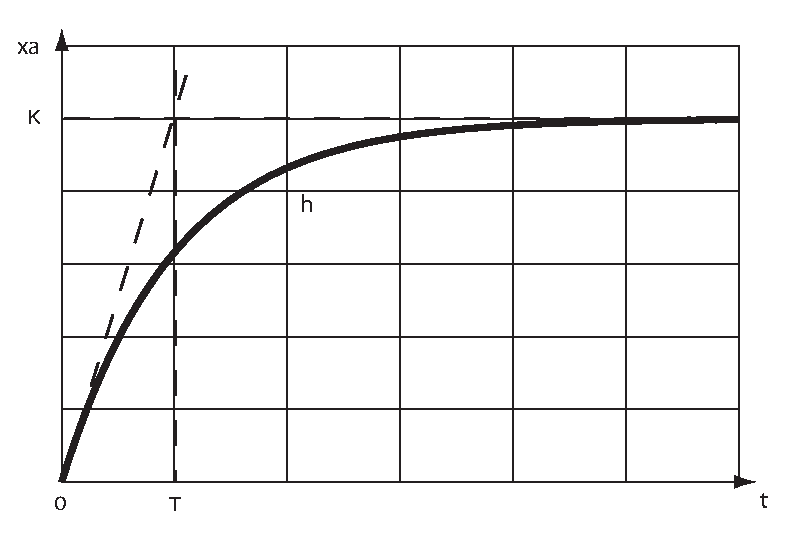
\includegraphics[width=0.6\textwidth]{figures/step_pt1.eps}
\caption[Boxplot]{Diese Abbildung zeigt eine Matlab-Darstellung, exportiert nach eps Force $F$ für die Bedingungen $A$, $B$, und $C$.}
\label{fig:boxplot}
\end{figure}

\paragraph{Beispiele für korrekte Achsenbeschriftungen}
\paragraph{Beispiel für formal falsche Achsenbeschriftung}

 
Tabellen sind mit Bildern vergleichbar, weshalb das zuvor Gesagte weitgehend auch für Tabellen gilt. Genau wie Bilder und Grafiken müssen auch Tabellen nummeriert werden. Üblich ist es, für Tabellen eine eigene Nummerierung zu verwenden, d.h. in einer Dokumentation gibt es möglicherweise eine Abbildung 1 und eine Tabelle 1.

\begin{table}[ht]
	%\centering\renewcommand{\arraystretch}{1.1} 
	\footnotesize
	\begin{tabularx}{0.9\textwidth}{llXXXXrr}
		\midrule
		\multicolumn{2}{c}{Bruchpunkte} & \multicolumn{4}{c}{Strukturbruchtermine} & 					\multicolumn{1}{c}{BIC}& \\
		\midrule
		\multicolumn{2}{c}{0}   				&       	&   	    &       	&	      	&	 -2.337& \\
		\multicolumn{2}{c}{1}    				& 03/2009 &     	  & 	      & 	      &  -2.369& \\
		\multicolumn{2}{c}{~\,2$^\star$}& 04/2007 & 03/2009 &   &   	    &  -2.395& \\
		\multicolumn{2}{c}{3}    				& 04/2006 & 03/2009 & 11/2010 &     	  &  -2.373& \\
		\multicolumn{2}{c}{4}    				& 07/2006 & 01/2008 & 07/2009 & 01/2011 &  -2.313& \\
		\midrule\\[-3mm]
		\multicolumn{8}{l}{\begin{minipage}{0.88\textwidth}Ergebnisse des CUSUM-Tests für monatliche \textsl{4TC+2Cal} FFA Log-Differenzen von 01/2005 - 12/2012. Die BIC-optimale Spezifikation ist durch $^\star$ gekennzeichnet.\end{minipage}}
	\end{tabularx}
	\caption{Ergebnisse des CUSUM Strukturbruchtests}
	\label{tab:cusum}
\end{table}

